\chapter{Elementos do texto} \label{cap:texto}

% - - - - - - - - - - - - - - - - - - - - - - - - - - - - - - - - - - -
\section{Figuras}\label{sec:figs} 

Rótulos de figuras e tabelas devem ser centralizados se tiverem até uma linha
(Figura~\ref{fig:exemploFig1}), caso contrário devem estar justificados e
identados em ambas as margens, como mostrado na Figura ~\ref{fig:exemploFig2}.
Essa formatação já é realizada automaticamente pela classe \textsf{imeufg}.

Os compiladores \LaTeX\ provêem um mecanismo bastante simples para inclusão de
figuras, o que pode ser feito com o auxílio de várias classes auxiliares (as
mais comuns são \verb|graphic| e \verb|graphicx|). A classe \verb|imeufg| usa o
comando \verb|\includegraphics|, da classe \verb|graphicx|, para a inclusão de
figuras e não é necessário você colocar a extensão do arquivo neste comando.
Por exemplo, para a figura \ref{fig:exemploFig1} os comandos usados foram:
\begin{Verbatim}
 \begin{figure}[htb]
  \centering
  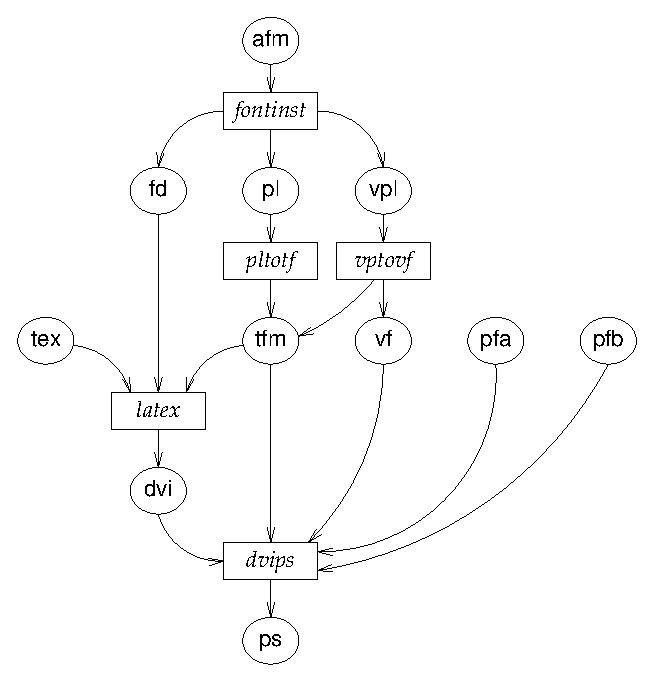
\includegraphics[width=0.40\textwidth]{./fig/01}
  \caption{Uma figura típica.}
  \label{fig:exemploFig1}
 \end{figure}
\end{Verbatim}

Ao se usar o compilador \LaTeX, as figuras podem estar nos formatos
\textit{eps} e \textit{ps}. Ao se usar o PDF\LaTeX, as figuras podem estar nos
formatos \textit{png}, \textit{jpg}, \textit{pdf} e \textit{mps}. A classe
\verb|graphicx| também pode ser usada para a inclusão de figuras, nos formatos
listados, ao se usar o PDF\LaTeX. Os comandos necessários são os mesmos ao se
incluir figuras ao se usar o compilador \LaTeX. O uso do comando
\verb|\includegraphics| faz com com que PDF\LaTeX\ procure primeiro por figuras
com extensão \textit{pdf}, depois \textit{jpg}, depois \textit{mps} e por
último \textit{png}. Aqui também não é necessário especificar a extensão do
arquivo.

Para a inclusão das figuras \ref{fig:exemploFig1} à \ref{fig:exemploFig3} os
comandos usados, tanto no \LaTeX\ quanto no PDF\LaTeX, seriam os mesmos. É
claro que em cada caso devem estar disponíveis as figuras nos formatos
suportados por cada compilador. Por exemplo, para a inclusão da figura
\ref{fig:exemploFig3} foram usados:
\begin{Verbatim}
 \begin{figure}[H]
  \centering
  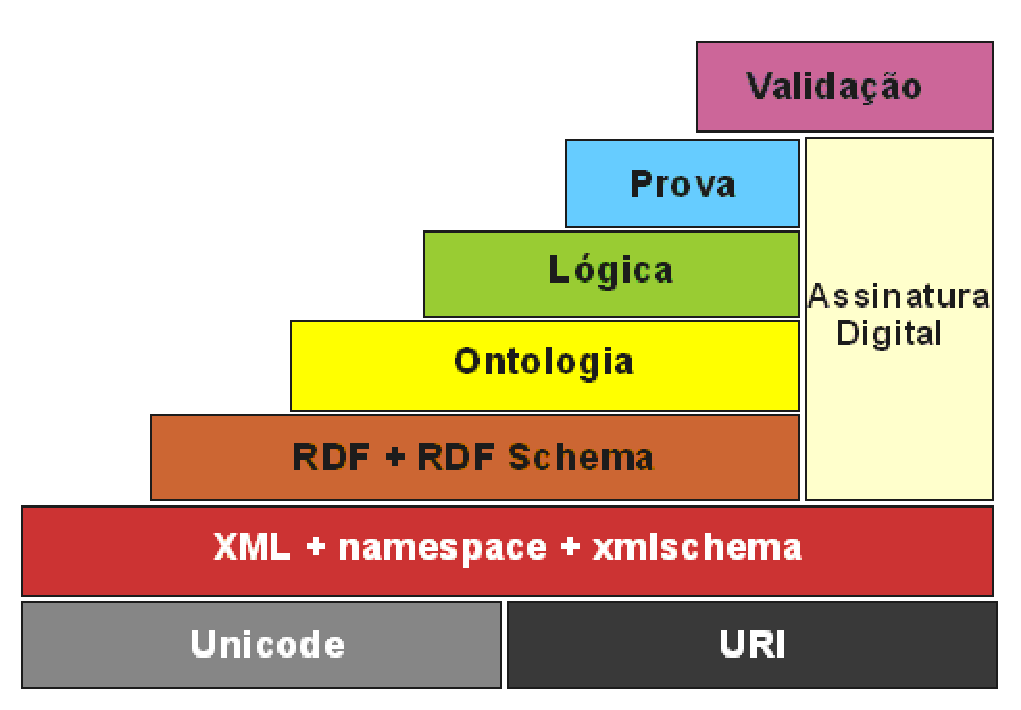
\includegraphics[width=0.40\textwidth]{./fig/03}
  \caption{Figura incluída no texto com a classe graphicx.}
  \label{fig:exemploFig3}
\end{figure}
\end{Verbatim}

\begin{figure}[H]
 \centering
  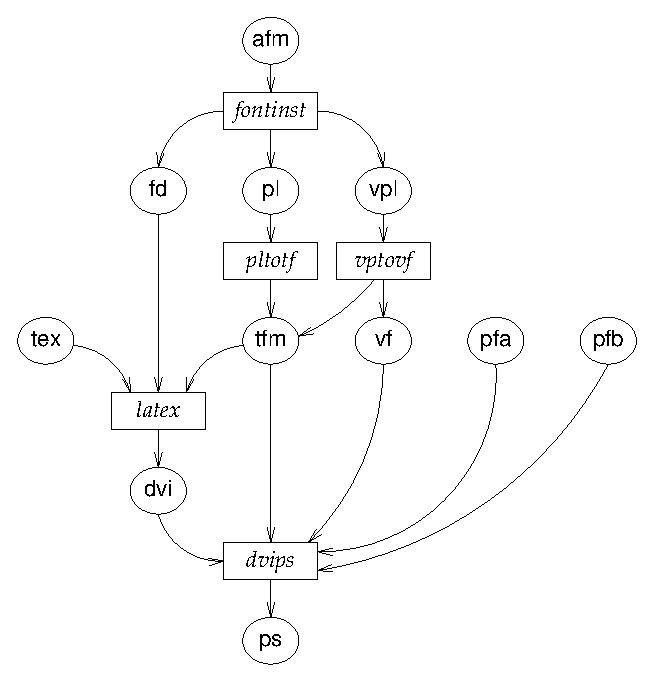
\includegraphics[width=0.40\textwidth]{./fig/01}
 \caption{Uma figura típica.}
 \label{fig:exemploFig1}
\end{figure}

\begin{figure}[H]
 \centering
 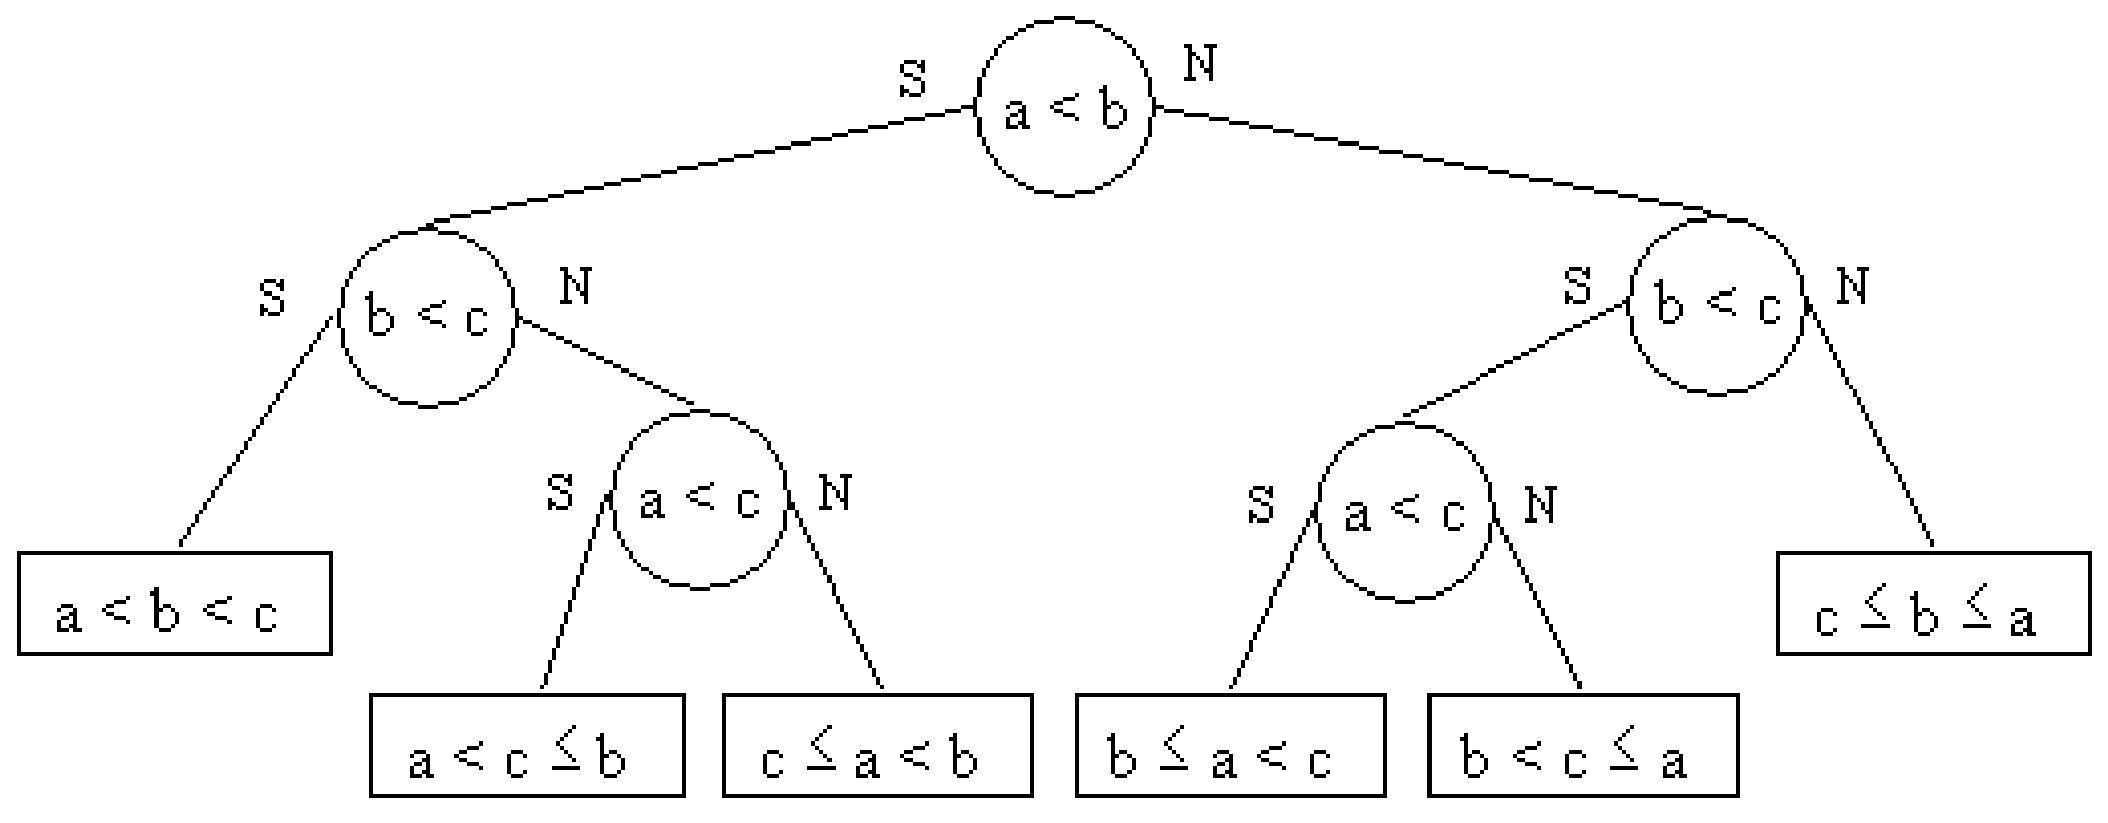
\includegraphics[width=0.30\textwidth]{./fig/02}
 \caption{Esta figura é um exemplo de um rótulo de figura que ocupa mais de uma linha, devendo ser identado e justificado.}
 \label{fig:exemploFig2}
\end{figure}

\begin{figure}[H]
 \centering
  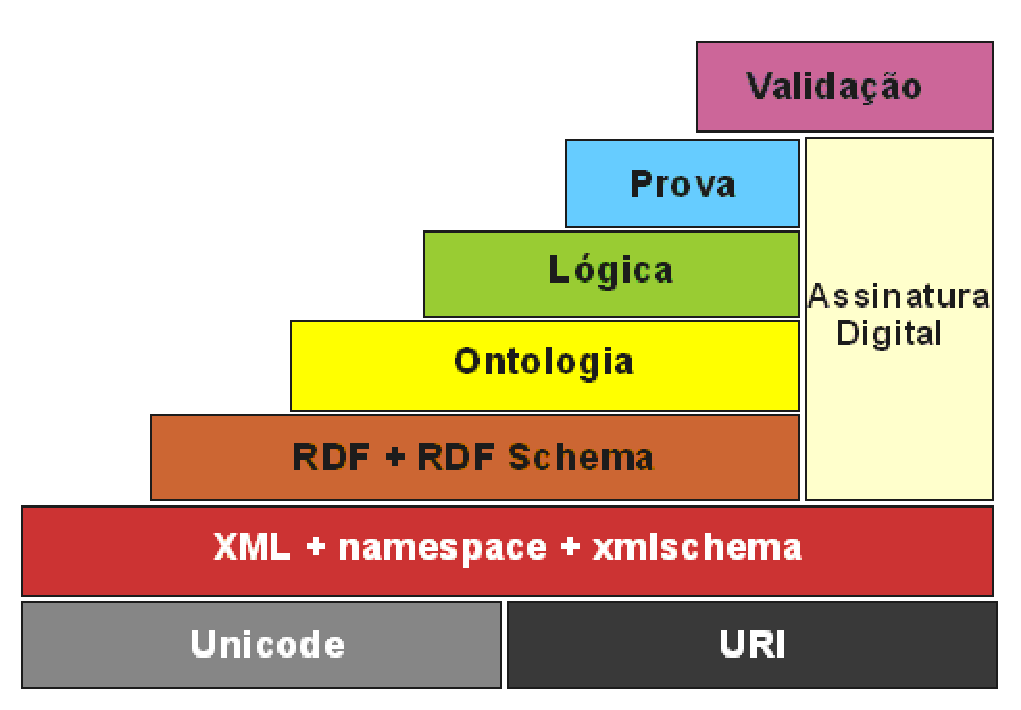
\includegraphics[width=0.40\textwidth]{./fig/03}
  \caption{Figura incluída no texto com a classe graphicx.}
 \label{fig:exemploFig3}
\end{figure}

\subsection{Subfiguras}
\label{subsec:subfigs} 
A classe \verb|subfigure| pode ser usada para a inclusão de figuras dentro de
figuras (consulte a documentação da classe para maiores detalhes). Por exemplo,
a Figura \ref{fig:subfiguras} contém duas subfiguras. Estas podem ser
referencidas por rótulos independentes, ou seja, podem ser referenciadas como
Figuras \ref{subfig:ex1} e \ref{subfig:ex2} ou Subfiguras \subref{subfig:ex1} e
\subref{subfig:ex2}.
\begin{figure}[h]
  \centering
  \subfigure[][Primeira subfigura.]
  {
    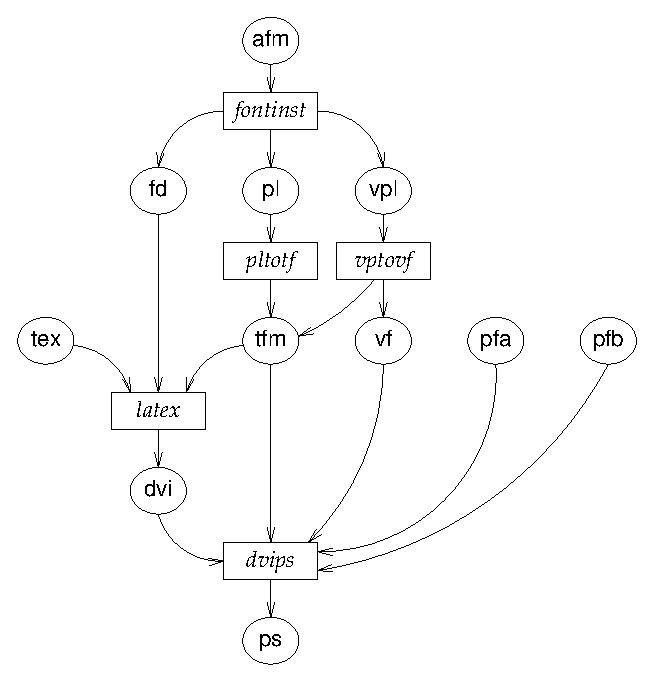
\includegraphics[width=0.35\textwidth]{./fig/01}
    \label{subfig:ex1}
  } \qquad
  \subfigure[Segunda subfigura (um pedaço).]
  {
    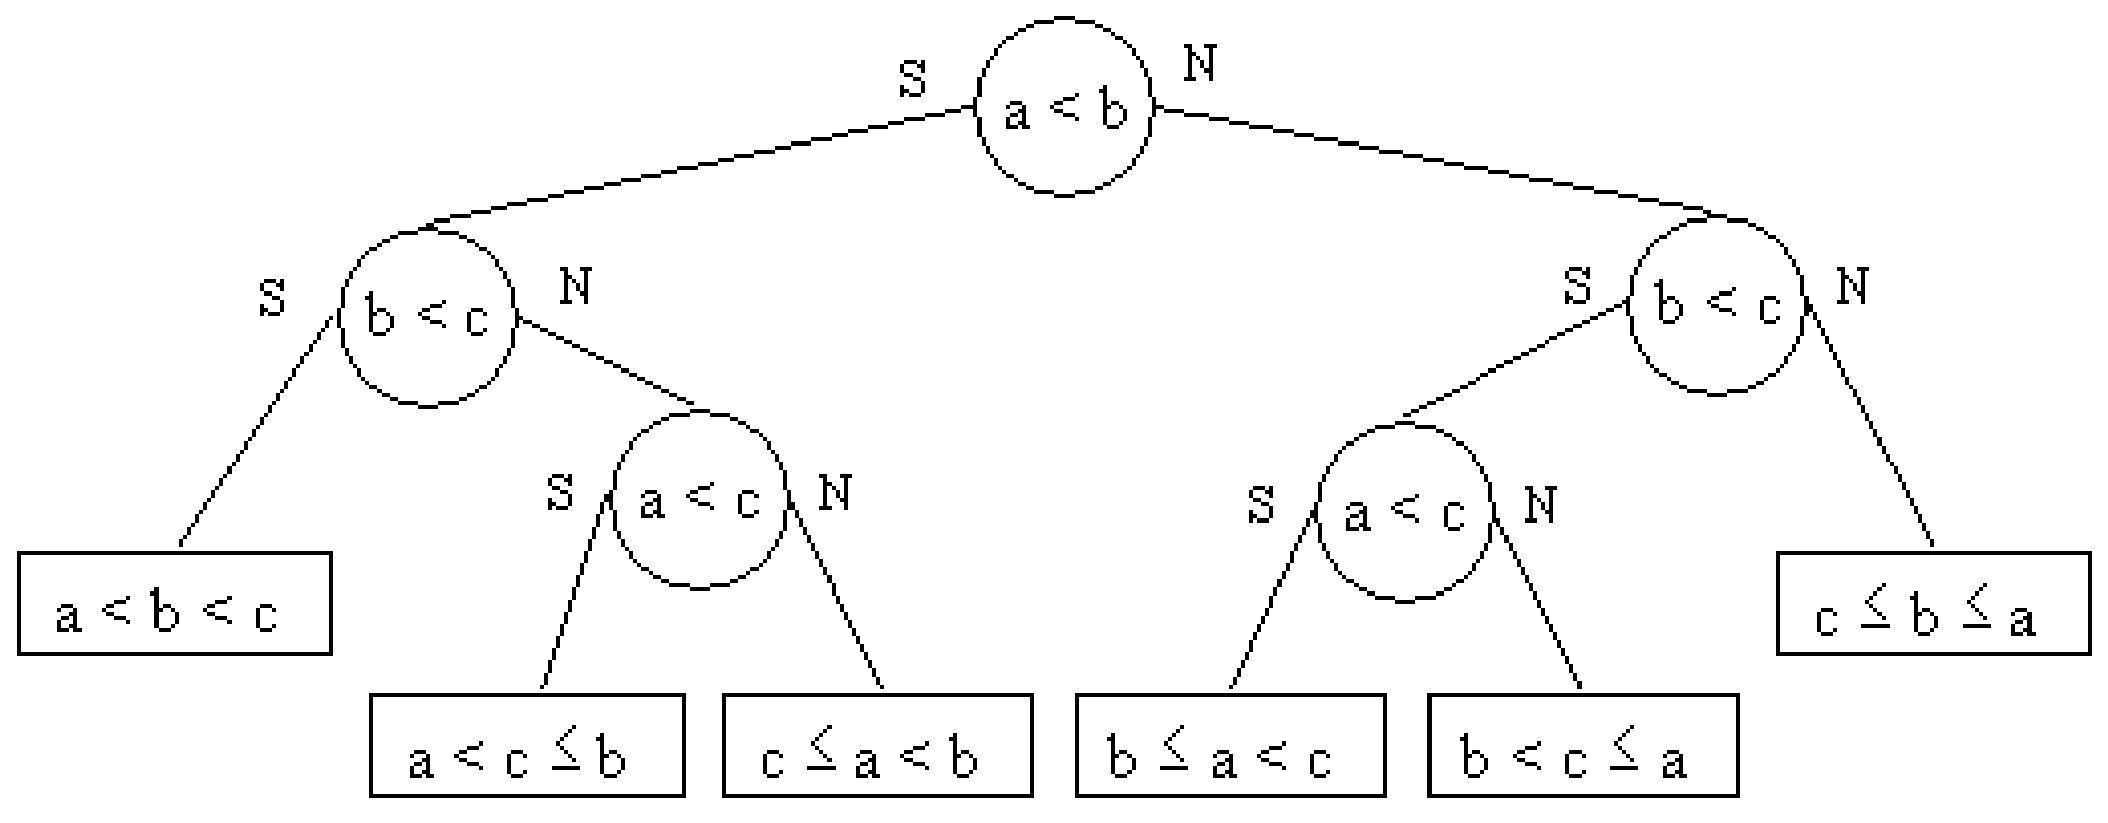
\includegraphics[width=0.30\textwidth]{./fig/02}
    \label{subfig:ex2}
  }
  \caption{{\subref{subfig:ex1}} e {\subref{subfig:ex2}} representam dois exemplos do uso de subfiguras dentro de uma única figura.}
  \label{fig:subfiguras}
\end{figure}

A figura \ref{fig:subfiguras} foi incluída com os comandos listados a seguir.
Observe que há rótulos independentes para cada uma das subfiguras e um rótulo
geral para a figura, os quais podem ser todos referenciados.
\begin{Verbatim}
\begin{figure}[h]
 \centering
  \subfigure[Primeira subfigura.]
   {
    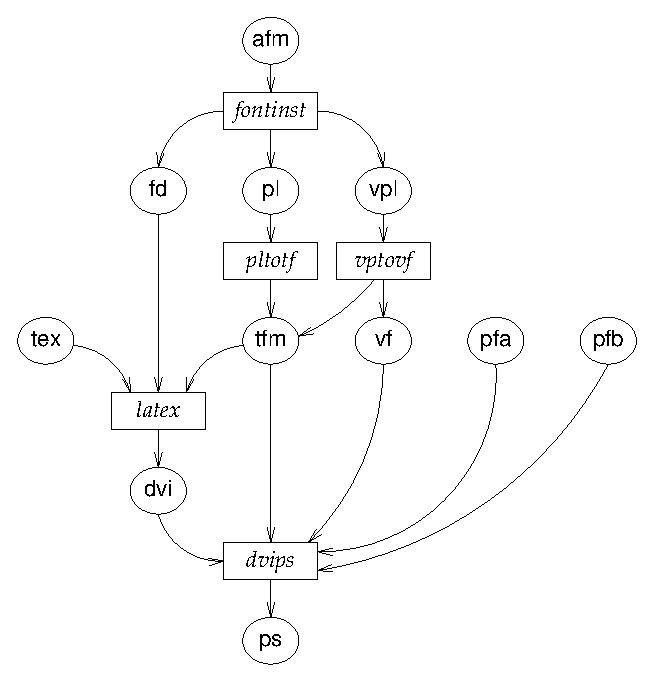
\includegraphics[width=0.35\textwidth]{./fig/01}
    \label{subfig:ex1}
   } \qquad
  \subfigure[Segunda subfigura (um pedaço).]
   {
    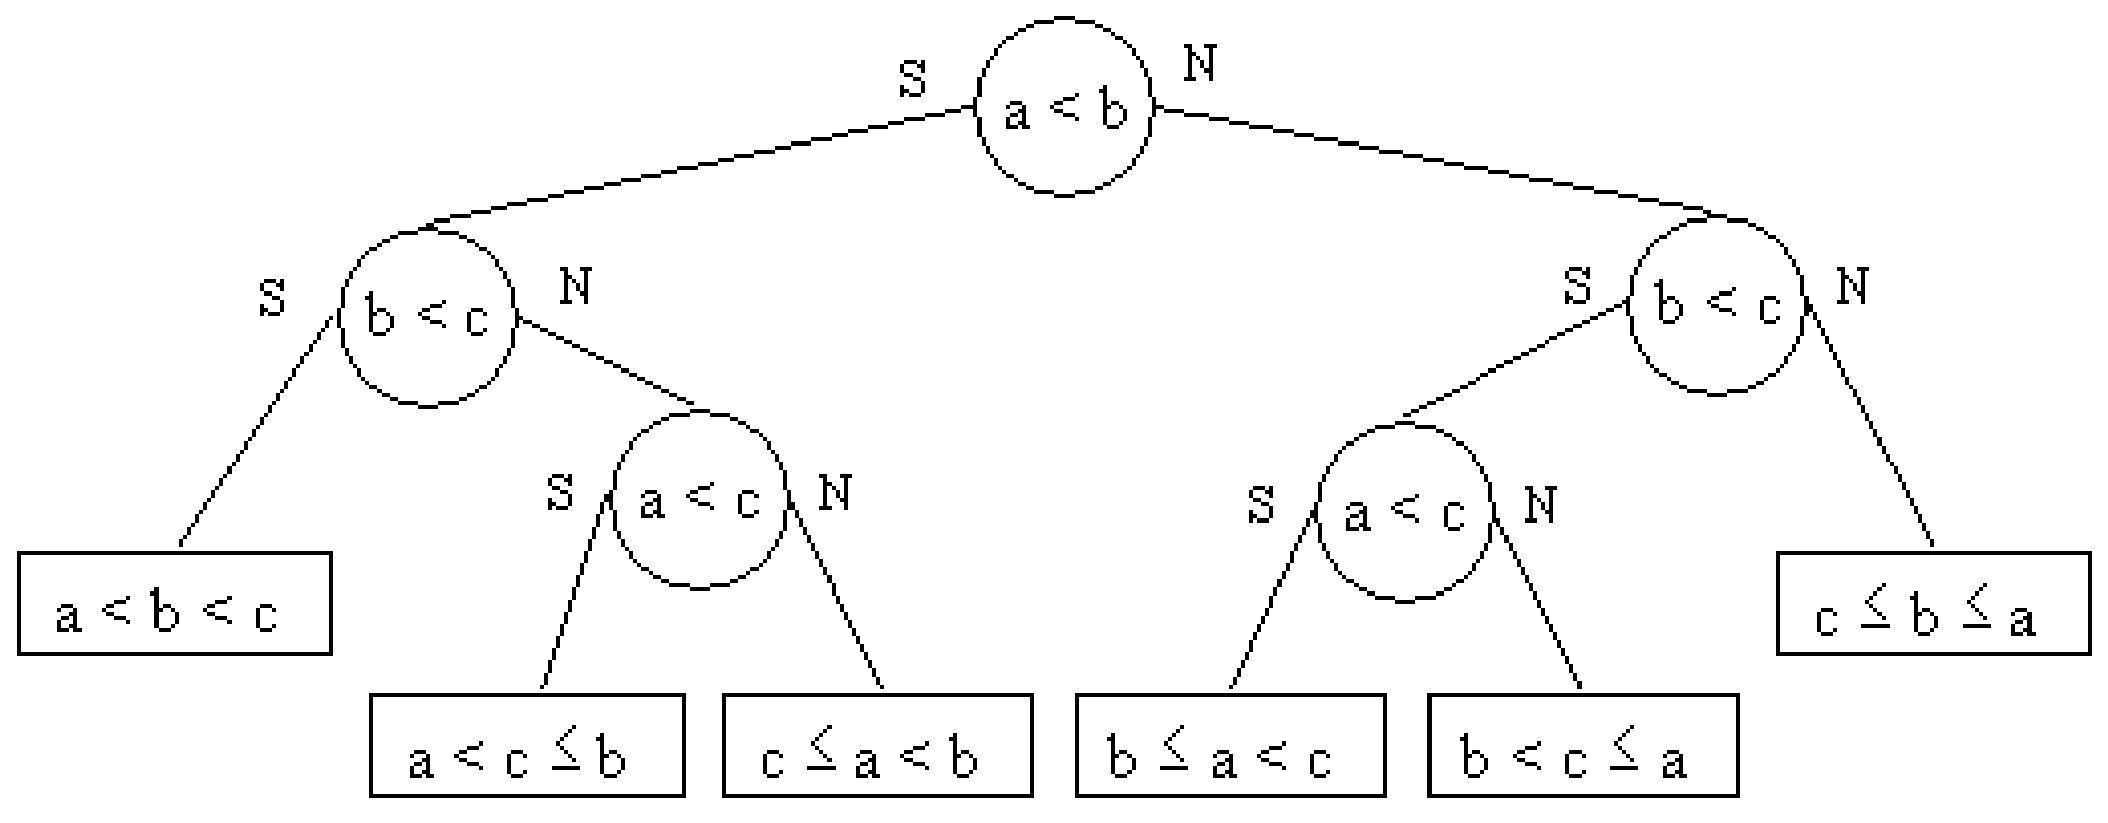
\includegraphics[width=0.30\textwidth]{./fig/02}
    \label{subfig:ex2}
   }
   \caption{{\subref{subfig:ex1}} e {\subref{subfig:ex2}} representam
             dois exemplos do uso de subfiguras dentro de uma única
             figura.}
  \label{fig:subfiguras}
\end{figure}
\end{Verbatim}
Caso uma subfiguras não tenha rótulo, para evitar que o apenas o número da
mesma apareça na Lista de Figuras, use o comando \verb|\subfigure[][]|.  Caso
uma subfigura tenha rótulo e deseja-se evitar que a mesma apareça na Lista de
Figuras, use o comando \verb|\subfigure[][Rótulo]|.

\section{Tabelas}\label{sec:tabs} 

Em tabelas, deve-se evitar usar cor de fundo diferente do branco e o uso de
linhas grossas ou duplas. Ao relatar dados empíricos, não se deve usar mais
dígitos decimais do aqueles que possam ser garantidos pela sua precisão e
reprodutibilidade. Rótulos de tabelas devem ser colocados antes das mesmas
(veja a Tabela \ref{tab:MarcMNem}).

\begin{table*}[hp]
  \centering
  \caption{Conteúdo do diretório \cite{Mar2004}}
  \label{tab:MarcMNem} 
  \begin{tabular}{|c|c|c|c|c|c|c|}
    \hline Tag & Comprimento & Início &  & Tag & Comprimento & Início \\
    \hline 001 & 0020        & 00000  &  & 100 & 0032        & 00235  \\
    \hline 003 & 0004        & 00020  &  & 245 & 0087        & 00267  \\
    \hline 005 & 0017        & 00024  &  & 246 & 0036        & 00354  \\
    \hline 008 & 0041        & 00041  &  & 250 & 0012        & 00390  \\
    \hline 010 & 0024        & 00082  &  & 260 & 0037        & 00402  \\
    \hline 020 & 0025        & 00106  &  & 300 & 0029        & 00439  \\
    \hline 020 & 0044        & 00131  &  & 500 & 0042        & 00468  \\
    \hline 040 & 0018        & 00175  &  & 520 & 0220        & 00510  \\
    \hline 050 & 0024        & 00193  &  & 650 & 0033        & 00730  \\
    \hline 082 & 0018        & 00217  &  & 650 & 0012        & 00763  \\
    \hline 
  \end{tabular} 
\end{table*}

\section{Algoritmos}\label{sec:algor} 

Algoritmos devem ser representados no formato do Algoritmo \ref{alg:poten}, que
foi descrito com o uso da classe \textsf{algorithm2e}. A rigor não é
obrigatório o uso dessa classe, contudo o uso da mesma permite que seja gerada
automaticamente uma lista de algoritmos logo após o sumário.

\medskip
\begin{center}
  \begin{minipage}{0.92\textwidth}
    \begin{algorithm2e}[H]
      \dontprintsemicolon
      \linesnumbered
      \SetLine
      \BlankLine
      \Entrada{vetor $A[i\,.\,.\,j]$, inteiros não negativos $i$ e $j$.}
      \Saida{vetor $A[i\,.\,.\,j]$ ordenado.}
      \BlankLine
      $n \leftarrow j - i$.\;
      \eSe{$(n<4)$}
      {Ordene com $\leq 3$ comparações.}
      {Divida $A$ em $\lceil\sqrt{n}\,\,\rceil$ subvetores de comprimento máximo $\lfloor\sqrt{n}\,\rfloor$.\;
      Aplique $MSR$ a cada um dos subvetores.\;
      Intercale os subvetores.\;}
      \caption{$MSR(A,i,j)$
      \label{alg:poten}}
    \end{algorithm2e}
  \end{minipage}
\end{center}

%% - - - - - - - - - - - - - - - - - - - - - - - - - - - - - - - - - - -
\section{Códigos de Programa}\label{sec:progs} 

Códigos de programa podem ser importados, mantendo-se a formatação original,
conforme se pode ver no exemplo do Código \ref{code:prog1}. Este exemplo usa o
ambiente \textsf{codigo}, definido na classe \textsf{imeufg}, que permite que
uma lista de programas seja gerada automaticamente logo após o sumário.

\begin{center}
 \begin{minipage}{0.7\textwidth}
  \begin{codigo}[H]
   \small
   \VerbatimInput[xleftmargin=10mm,numbers=left,obeytabs=true]{./prog/insertionsort.c}
   \caption{\texttt{insertionsort()}}
   \label{code:prog1}
  \end{codigo}
 \end{minipage}
\end{center}

%% - - - - - - - - - - - - - - - - - - - - - - - - - - - - - - - - - - -
\section{Teoremas, Corolários e Demonstrações}\label{sec:teor}

O uso do ambiente \textsf{theorem} permite a escrita de teoremas, como no
exemplo a seguir:

\begin{verbatim}
\begin{theorem}[Pitágoras]
Em todo triângulo retângulo o quadrado do comprimento
da hipotenusa é igual a soma dos quadrados dos
comprimentos dos catetos.
\end{theorem}
\end{verbatim}

O resultado é o mostrado a seguir:

\begin{theorem}[Pitágoras]
Em todo triângulo retângulo o quadrado do comprimento da hipotenusa é igual a
  soma dos quadrados dos comprimentos dos catetos.
\end{theorem}

Da mesma forma pode-se usar o ambiente \textsf{proof} para demonstrações de teoremas:
\begin{verbatim}
\begin{proof}
Para demonstrar o Teorema de Pitágoras \dots
\end{proof}
\end{verbatim}

Neste caso, o resultado é:
\begin{proof}
Para demonstrar o Teorema de Pitágoras \dots
\end{proof}

Além desses dois ambientes, estão definidos os ambientes \textsf{definition}
(Definição), \textsf{corollary} (Corolário), \textsf{lemma} (Lema)),
\textsf{proposition} (Proposição), \textsf{comment} (Observação).

\section{Citações Longas}\label{sec:citacoes}

Segundo as normas da ABNT, uma citação longa (mais de 3 linhas) deve seguir uma
formação especial. Para tanto foi criado o ambiente \verb|citacao|, o qual é
baseado no ambiente de mesmo nome definido pelo grupo ABNTex
\cite{abnt-classe-doc}:

\begin{citacao}
  Uma citação longa (mais de 3 linhas) deve vir em parágrafo separado, com
  recuo de 4cm da margem esquerda, em fonte menor, sem as aspas
  \cite[4.4]{NBR10520:2001} e com espaçamento simples
  \cite[5.3]{NBR14724:2001}. Uma regra de como fazer citações em geral não é
  simples. É prudente ler \cite{NBR10520:2001} se você optar for fazer uso
  freqüente de citações. Para satisfazer às exigências tipográficas que a norma
  pede para citações longas, use o ambiente citacao.
\end{citacao}

Este exemplo de citação longa foi produzido com o uso do ambiente
\verb|citacao|, como descrito logo a seguir:

\begin{verbatim}
\begin{citacao}
Uma citação longa (mais de 3 linhas) deve vir em parágrafo
separado, com recuo de 4cm da margem esquerda, em fonte menor,
sem as aspas \cite[4.4]{NBR10520:2001} e com espaçamento
simples \cite[5.3]{NBR14724:2001}. Uma regra de como fazer
citações em geral não é simples. É prudente ler
\cite{NBR10520:2001} se você optar for fazer uso freqüente
de citações. Para satisfazer às exigências tipográficas que a
norma pede para citações longas, use o ambiente citacao.
\end{citacao}
\end{verbatim}

\section{Referências Bibliográficas}\label{sec:refs} 

Esta seção mostra exemplos de uso de referências bibliográficas com \BibTeX{} e
do comando \verb|\cite|.  Muitas das entradas listadas na
página~\pageref{ref-bib} foram obtidas de:
\href{http://liinwww.ira.uka.de/bibliography/index.html}{http://liinwww.ira.uka.de/bibliography/index.html}.
Outro grande repositório de referências já em formato \BibTeX{} está disponível
em:
\href{http://www.math.utah.edu/~beebe/bibliographies.html}{http://www.math.utah.edu/~beebe/bibliographies.html}.

As referências bibliográficas devem ser não ambíguas e uniformes. Recomenda-se
usar números entre colchetes, como por exemplo \cite{SmiJon1999},
\cite{Knu1989} e \cite{LeeSwi2002}. O comando \verb|\nocite| não produz texto,
mas permite que a entrada seja incluída nas referências. Por exemplo, o comando
\verb|\nocite{Ber1970}| gera na lista de referências bibliográficas a entrada
referente à chave \textsf{Ber1970}, mas não inclui nenhuma referência no texto.
O comando \verb|\nocite{*}| faz com que todas as entradas do arquivo de dados
do \BibTeX{} sejam incluídas nas referências. \nocite{Ber1970}

Existem vários livros sobre \LaTeX{}, como \cite{Bue1990,Hah1991,KopDal1995},
embora os mais famosos sejam sem dúvida \cite{Lam1996} e \cite{GooMitSam1994}.
Para converter documentos \LaTeX{} para HTML veja \cite[pg.1--10]{Dra1994}.
